\documentclass[aspectratio=169,11pt,hyperref={colorlinks=true}]{beamer}
\usetheme{boxes}
\setbeamertemplate{navigation symbols}{}
\definecolor{ibm}{RGB}{70,107,176}
\setbeamercolor{titlelike}{fg=ibm}
\setbeamercolor{structure}{fg=ibm}
\hypersetup{colorlinks,urlcolor=ibm}
\setbeamertemplate{footline}[frame number]
% Inserting graphics
\usepackage{graphicx}
% Side-by-side figures, etc
\usepackage{subfigure}
% Code snippits
\usepackage{listings}
% Color stuff
\usepackage{color}
\usepackage{amsmath}
\usepackage{tikz}
\usepackage{tipa}
\newcommand\RBox[1]{%
  \tikz\node[draw,rounded corners,align=center,] {#1};%
}
\newcommand{\light}[1]{\textcolor{gray}{#1}}
\usepackage{hyperref}
%\usecolortheme{buzz}
%\usecolortheme{wolverine}
%\usetheme{Boadilla}
\usepackage[T1]{fontenc}
\usepackage{animate}
\usepackage{pgfplotstable}
\usepackage{colortbl}
\usepackage{booktabs}

\definecolor{mygreen}{rgb}{0,0.6,0}
\definecolor{mygray}{rgb}{0.5,0.5,0.5}
\definecolor{mymauve}{rgb}{0.58,0,0.82}

\pgfplotstableset{col sep=comma, header=has colnames}

\lstset{ %
  backgroundcolor=\color{white},   % choose the background color; you must add \usepackage{color} or \usepackage{xcolor}
  breakatwhitespace=false,         % sets if automatic breaks should only happen at whitespace
  breaklines=true,                 % sets automatic line breaking
  captionpos=b,                    % sets the caption-position to bottom
  commentstyle=\color{ibm},        % comment style
  extendedchars=true,              % lets you use non-ASCII characters; for 8-bits encodings only, does not work with UTF-8
  keepspaces=true,                 % keeps spaces in text, useful for keeping indentation of code (possibly needs columns=flexible)
  keywordstyle=\color{blue},       % keyword style
  otherkeywords={*,...},           % if you want to add more keywords to the set
  numbersep=5pt,                   % how far the line-numbers are from the code
  numberstyle=\tiny\color{mygray}, % the style that is used for the line-numbers
  rulecolor=\color{black},         % if not set, the frame-color may be changed on line-breaks within not-black text (e.g. comments (green here))
  showspaces=false,                % show spaces everywhere adding particular underscores; it overrides 'showstringspaces'
  showstringspaces=false,          % underline spaces within strings only
  showtabs=false,                  % show tabs within strings adding particular underscores
  stringstyle=\color{ibm},         % string literal style
}

\setbeamerfont{caption}{series=\normalfont,size=\fontsize{8}{10}}
\setbeamertemplate{caption}{\raggedright\insertcaption\par}

\setlength{\abovecaptionskip}{0pt}
\setlength{\floatsep}{0pt}

\author[Andrea]{%
   \texorpdfstring{
       \begin{columns}
           \column{.45\linewidth}
           \centering
           Andrea Frittoli\\
           \href{mailto:andrea.frittoli@gmail.com}{andrea.frittoli@gmail.com}\\
       \end{columns}
  }
  {Andrea Frittoli}
}

\date{September 12, 2018}

\title[Community before Code
\hspace{2em}\insertframenumber/\inserttotalframenumber]{Community before Code}

\begin{document}

{
\setbeamertemplate{background canvas}{
\includegraphics[width=\paperwidth,height=\paperheight]{_backgrounds/black_bg.png}}
\setbeamertemplate{footline}{}
\begin{frame}[noframenumbering]
    \setbeamercolor{titlelike}{fg=white}
    \setbeamercolor{structure}{fg=white}
    \setbeamercolor{normal text}{fg=white}
    \hypersetup{colorlinks,urlcolor=white}
    \setbeamercolor{author}{fg=white}
    \setbeamercolor{date}{fg=white}
    \setbeamercolor{background}{bg=ibm}
    \titlepage{}
    \centering
    \href{https://github.com/afrittoli/community\_before\_code\_talk}{https://github.com/afrittoli/community\_before\_code\_talk}
\end{frame}
}

\usebackgroundtemplate{%
  
\includegraphics[width=\paperwidth,height=\paperheight]{_backgrounds/white_bg.png}}

\section{Intro}
\begin{frame}[c]
  \frametitle{An Open Source Talk}
    \begin{overlayarea}{\textwidth}{.2\textheight}
      \begin{itemize}
          \uncover<1->{\item{It's on \href{https://github.com/afrittoli/community\_before\_code\_talk}{GitHub}}}
          \uncover<2->{\item{Apache 2.0 \& Creative Commons}}
      \end{itemize}
    \end{overlayarea}
    \begin{figure}
      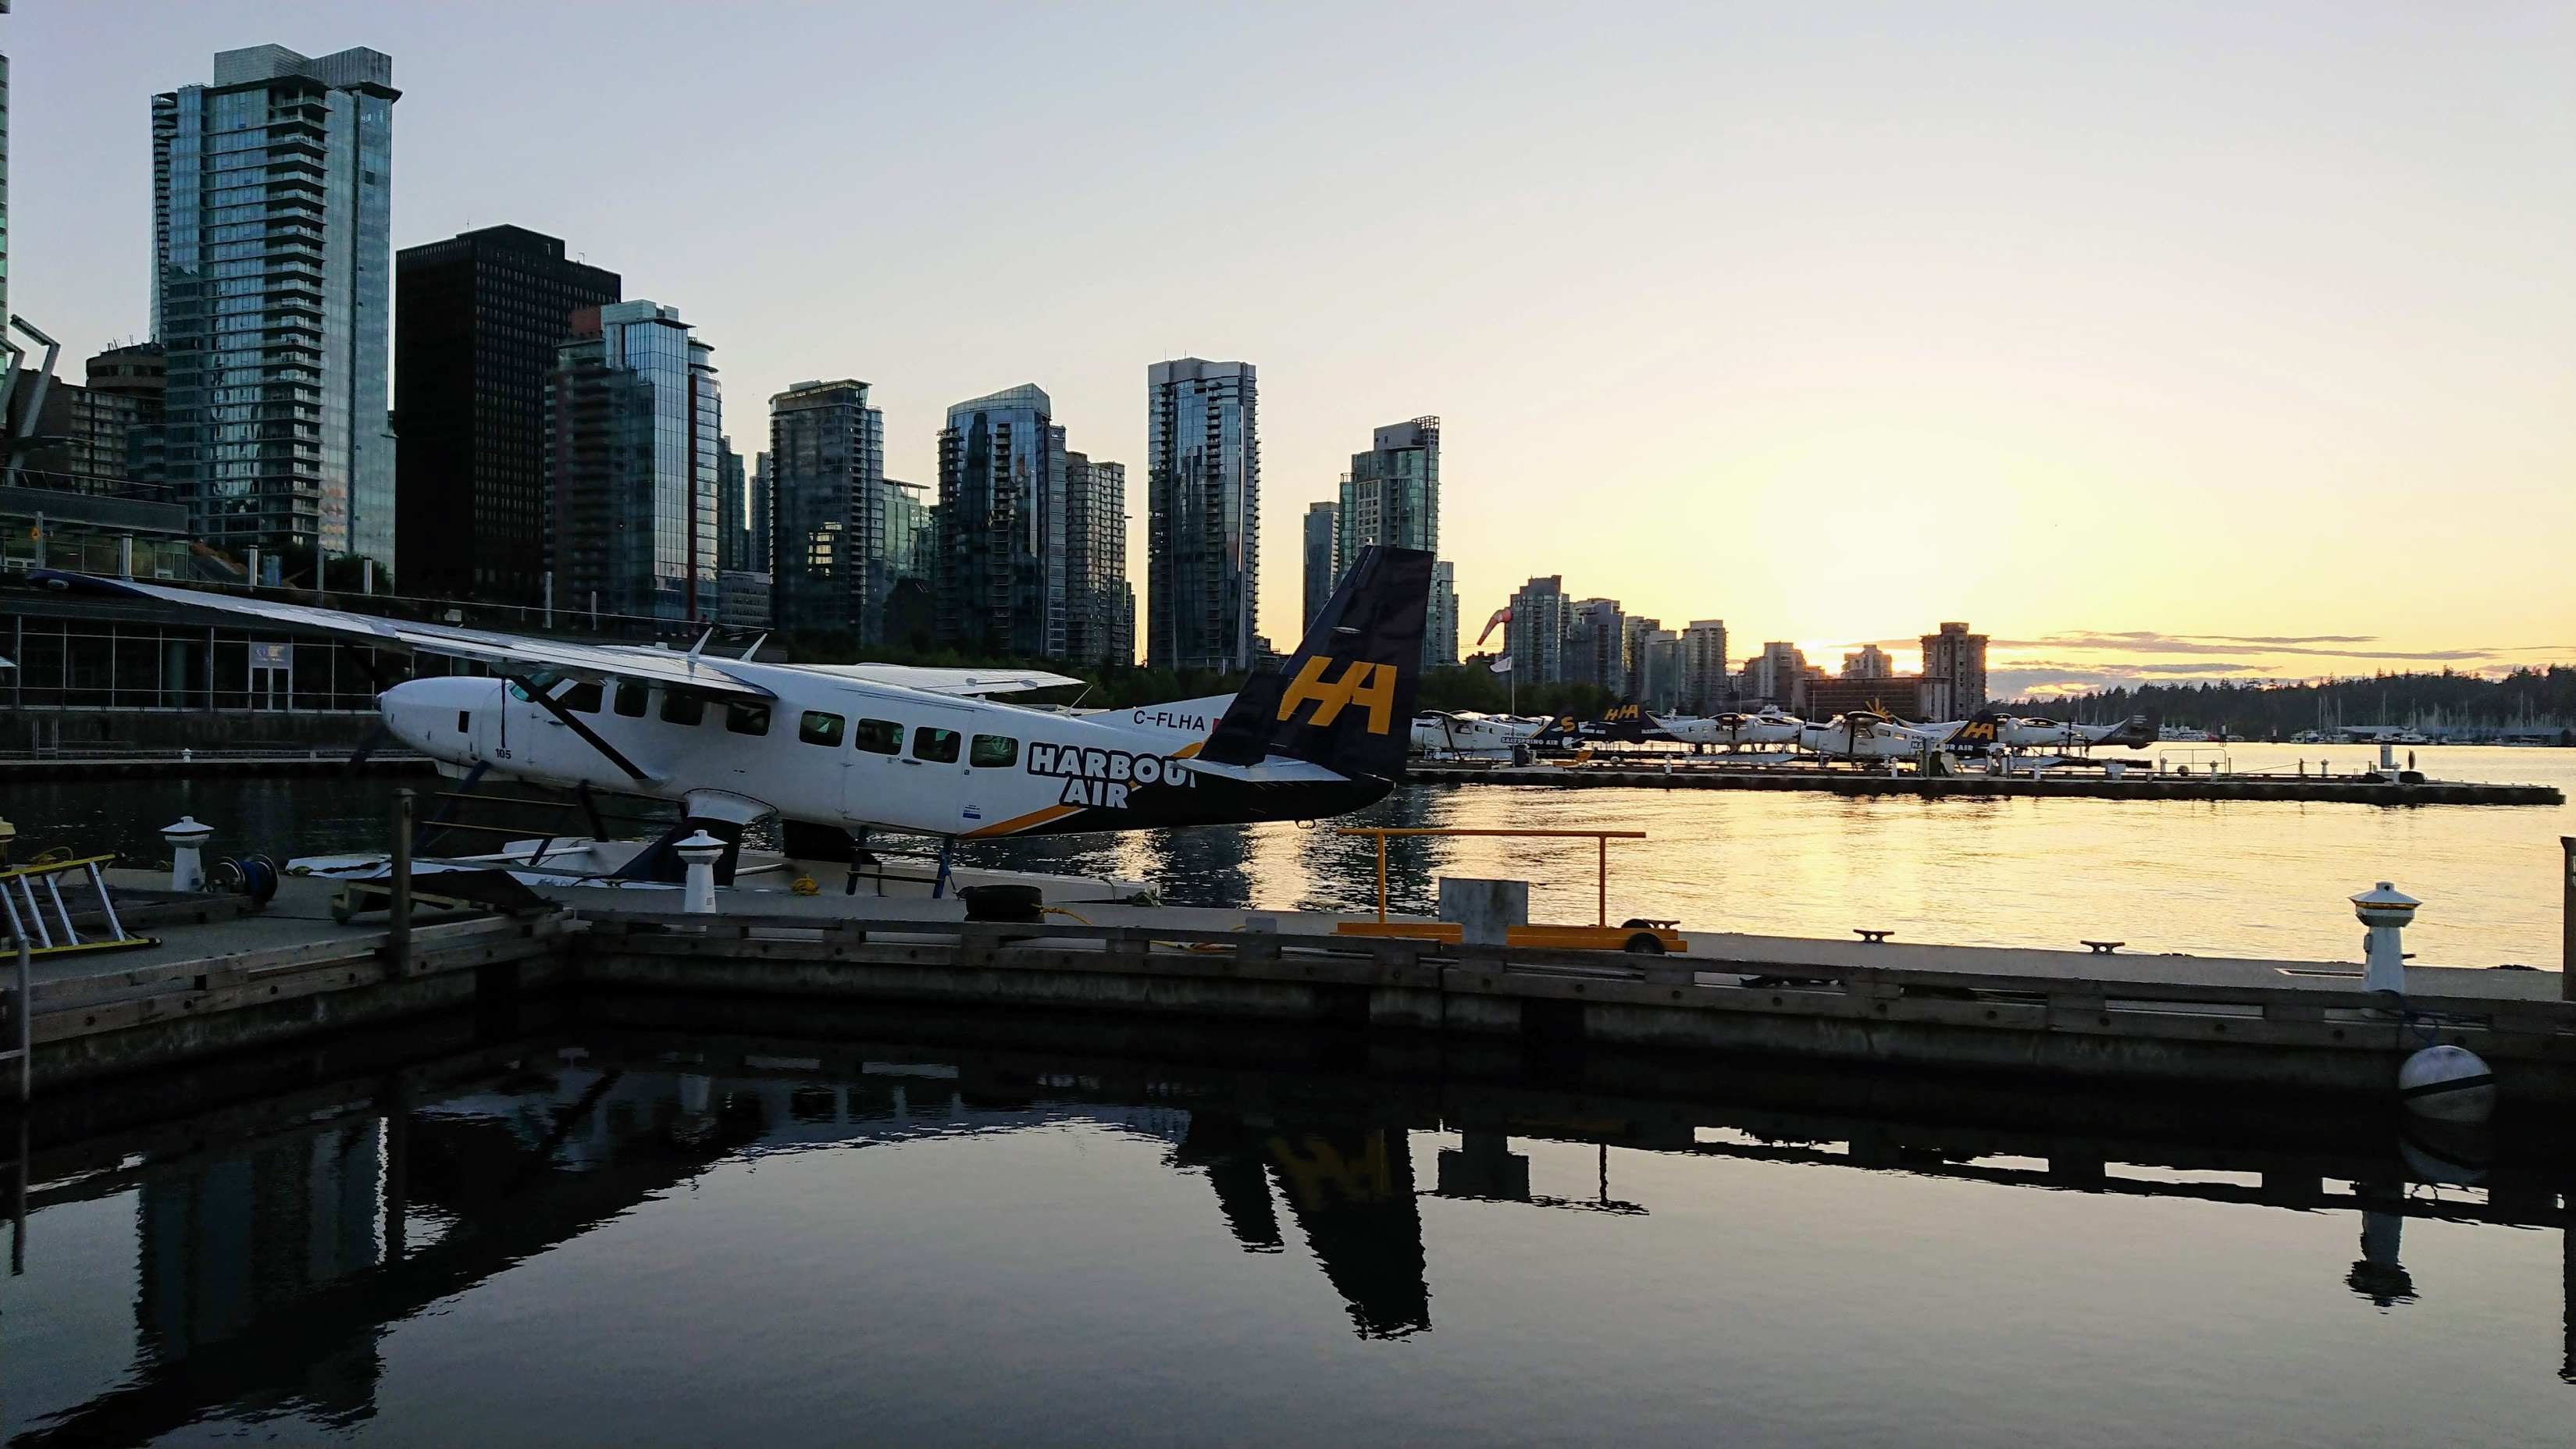
\includegraphics[width=0.6\textwidth]{pictures/vancouver_harbour_plane.jpg}
         \uncover<2->{\caption{"Sea Plane in Vancouver" by \href{https://andreafrittoli.me}{Andrea Frittoli} under \href{https://creativecommons.org/licenses/by/2.0/}{CC BY 2.0}}}
    \end{figure}
\end{frame}

\begin{frame}
  \frametitle{Reusing an Open Source Talk}
    \begin{overlayarea}{\textwidth}{.3\textheight}
      \begin{itemize}
          \item{New conference, new version}
          \item{Old version is never updated}
          \item{Single contributor (or small group)}
      \end{itemize}
    \end{overlayarea}
    \begin{figure}
      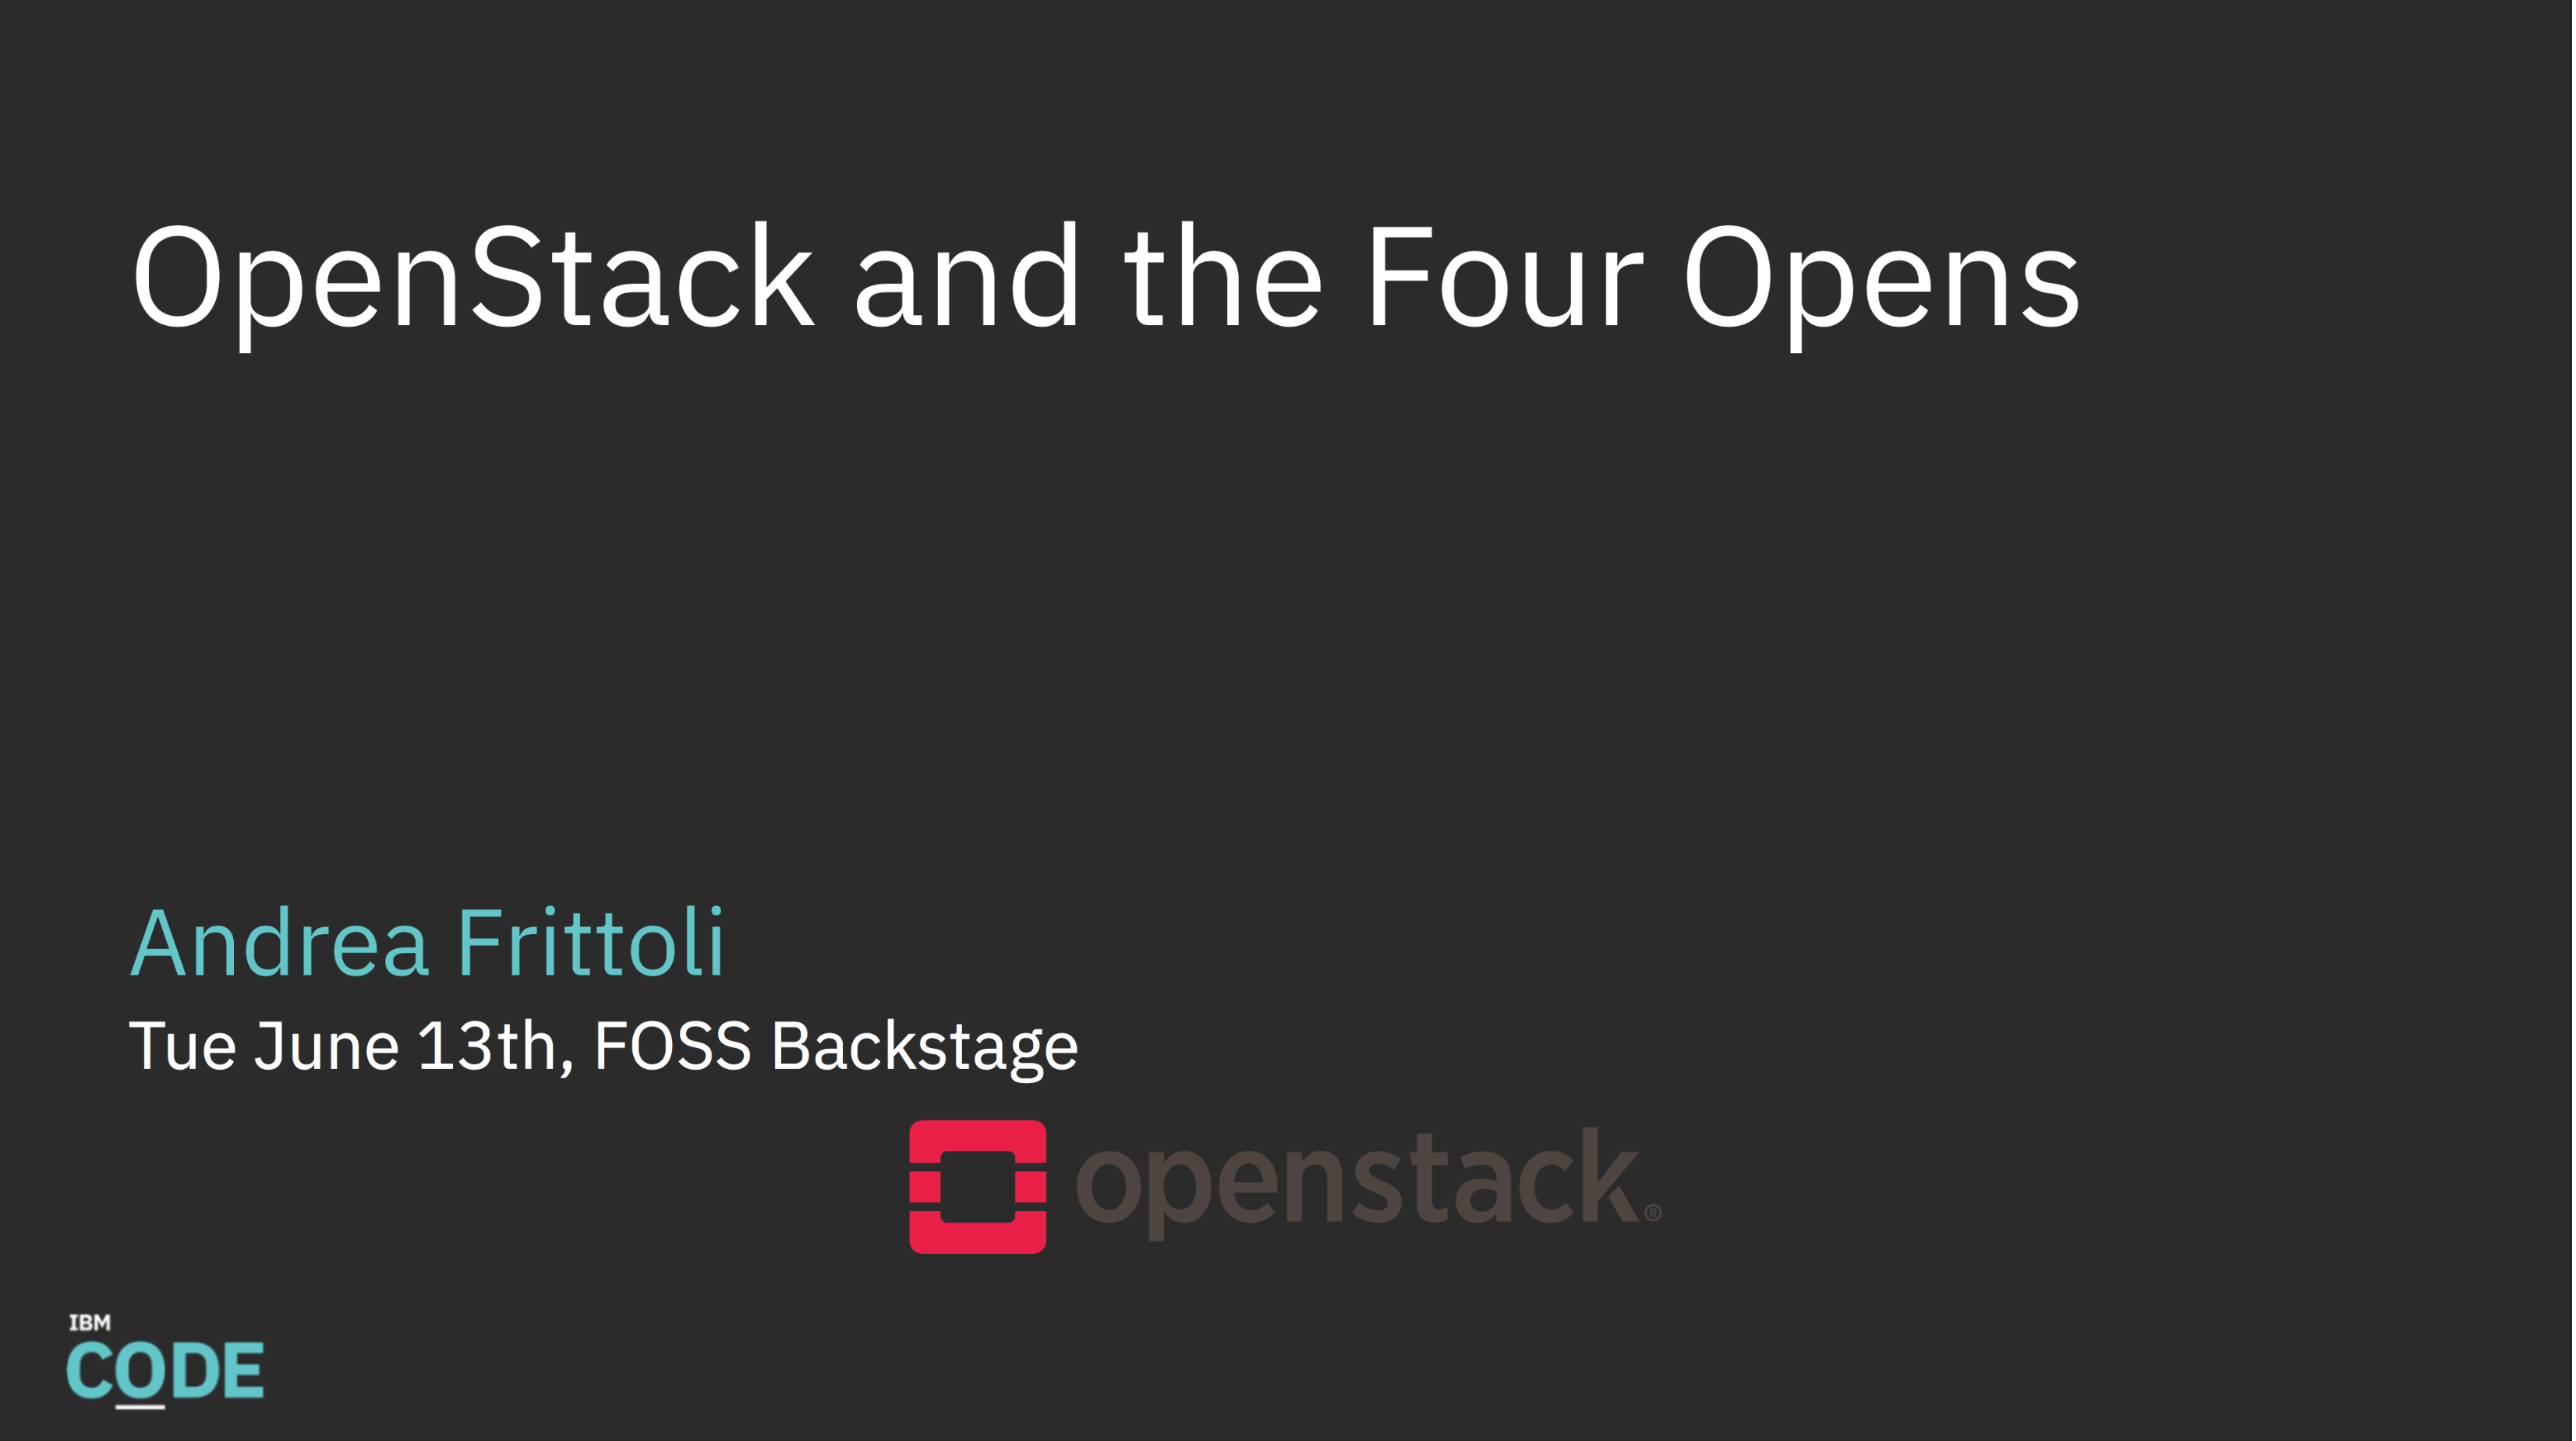
\includegraphics[width=0.4\textwidth]{pictures/old_presentation.png}
         \caption{"OpenStack and the Four Opens" by \href{https://afrittoli.github.io/openstack-four-opens/}{Andrea Frittoli} under \href{https://creativecommons.org/licenses/by/2.0/}{CC BY 2.0}}
    \end{figure}
\end{frame}

\begin{frame}
  \frametitle{Reusing Software}
    \begin{itemize}
        \item{Can I contribute?}
        \item{Is the API stable?}
        \item{Can I influence the design?}
        \item{How do I get involved?}
    \end{itemize}
\end{frame}

\section{OpenStack}
\begin{frame}
  \frametitle{A bit of history}
  \begin{columns}
    \column{0.5\linewidth}
      \begin{itemize}
          \item{2010: Rackspace and NASA create OpenStack}
          \item{2012: OpenStack Foundation}
          \item{2014: "The Big Tent"}
      \end{itemize}
    \column{0.5\linewidth}
      \begin{figure}
      \begin{center}
        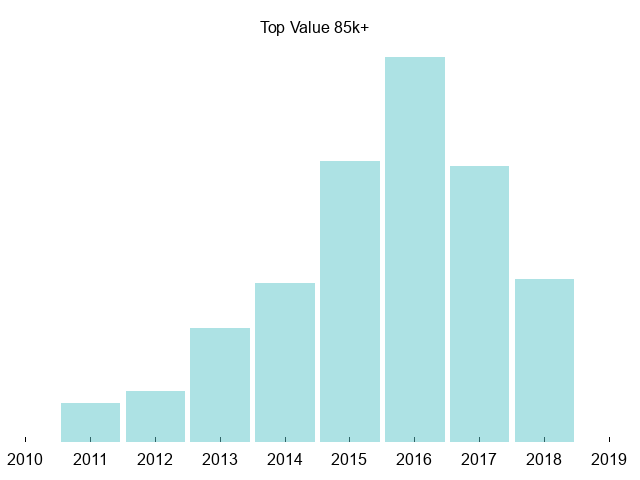
\includegraphics[width=1\textwidth]{graphs/commits.png}
           \caption{Commits/year - Source: stackalytics.com}
      \end{center}
      \end{figure}
  \end{columns}
\end{frame}

\begin{frame}
  \frametitle{The OpenStack way}
  \begin{columns}
    \column{0.4\linewidth}
      \begin{itemize}
          \item{Open Source}
          \item{Open Design}
          \item{Open Development}
          \item{Open Community}
      \end{itemize}
    \column{0.6\linewidth}
      \begin{figure}
      \begin{center}
        
\includegraphics[width=0.4\textwidth]{pictures/OpenStack-Logo-Mark.png}
      \end{center}
      \end{figure}
  \end{columns}
\end{frame}

\section{Opens}
\begin{frame}
  \frametitle{Open Source}
    \begin{itemize}
        \item{...}
    \end{itemize}
\end{frame}

\begin{frame}
  \frametitle{Open Design}
    \begin{itemize}
        \item{...}
    \end{itemize}
\end{frame}

\begin{frame}
  \frametitle{Open Design}
    \begin{itemize}
        \item{...}
    \end{itemize}
\end{frame}

\begin{frame}
  \frametitle{Open Development}
    \begin{itemize}
        \item{...}
    \end{itemize}
\end{frame}

\begin{frame}
  \frametitle{Open Development}
    \begin{itemize}
        \item{...}
    \end{itemize}
\end{frame}

\begin{frame}
  \frametitle{Open Community}
    \begin{itemize}
        \item{...}
    \end{itemize}
\end{frame}

\begin{frame}
  \frametitle{Open Community}
    \begin{itemize}
        \item{...}
    \end{itemize}
\end{frame}

\begin{frame}
  \frametitle{Open Community}
    \begin{itemize}
        \item{...}
    \end{itemize}
\end{frame}

\section{Culture}

\begin{frame}
  \frametitle{Principles}
    \begin{itemize}
        \item{...}
    \end{itemize}
\end{frame}

\begin{frame}
  \frametitle{Principles}
    \begin{itemize}
        \item{...}
    \end{itemize}
\end{frame}

\begin{frame}
  \frametitle{Principles}
    \begin{itemize}
        \item{...}
    \end{itemize}
\end{frame}

\section{Conclusions}

\begin{frame}
  \frametitle{References}
  \begin{itemize}
      \item{This talk: \href{https://github.com/afrittoli/community\_before\_code\_talk}{https://github.com/afrittoli/community\_before\_code\_talk}}
  \end{itemize}
\end{frame}

\section{Questions}
\begin{frame}[c]
    %\frametitle{Questions?}
    \begin{center}
        \Huge Thank you!\\Questions?
    \end{center}
\end{frame}

\end{document}
